\documentclass[tikz,border=7pt]{standalone}

\usepackage{amsmath}
\usepackage{tikz}
\usetikzlibrary{arrows.meta}

\begin{document}
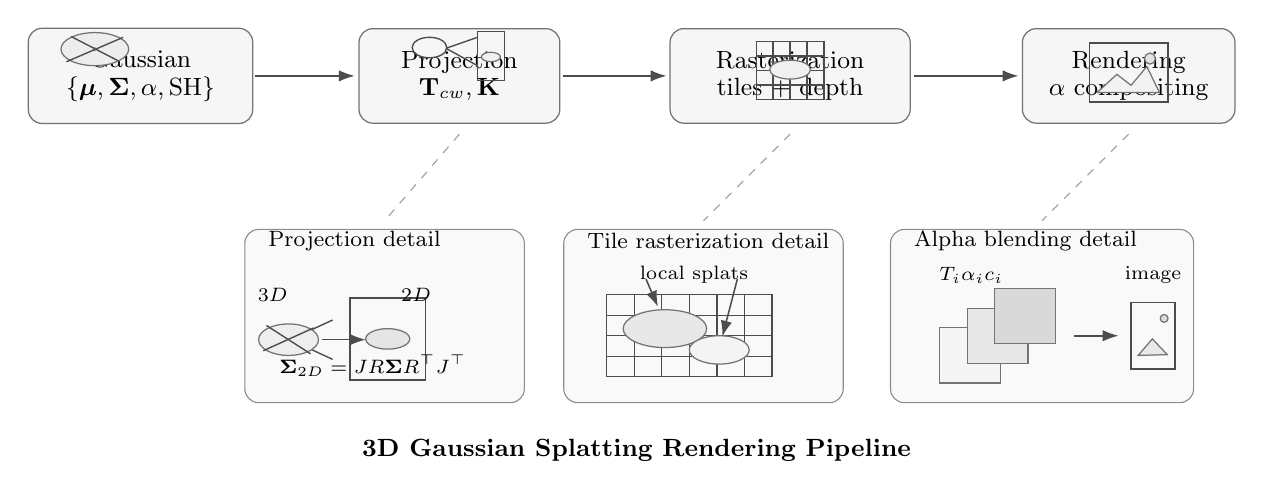
\begin{tikzpicture}[
    font=\small,
    mainbox/.style={
        rounded corners=5pt,
        draw=black!55,
        line width=0.45pt,
        fill=gray!7,
        align=center,
        inner xsep=9pt,
        inner ysep=8pt
    },
    detailbox/.style={
        rounded corners=5pt,
        draw=black!45,
        line width=0.4pt,
        fill=gray!5,
        align=center,
        inner xsep=7pt,
        inner ysep=7pt
    },
    arrow/.style={
        -{Latex[length=2.0mm,width=1.45mm]},
        draw=black!70,
        line width=0.55pt
    },
    guide/.style={
        draw=black!35,
        line width=0.45pt,
        dashed
    },
    ink/.style={
        draw=black!70,
        line width=0.5pt
    },
    soft/.style={
        draw=black!55,
        line width=0.45pt,
        fill=gray!12
    }
]

% ---------------------------------------------------------------------------
% Main pipeline: compact high-level flow
% ---------------------------------------------------------------------------
\node[mainbox, minimum width=2.85cm, minimum height=1.20cm] (gauss) at (0.00,0.00)
    {Gaussian\\[-1pt]$\{\boldsymbol{\mu},\boldsymbol{\Sigma},\alpha,\mathrm{SH}\}$};
\node[mainbox, minimum width=2.55cm, minimum height=1.20cm] (proj) at (4.05,0.00)
    {Projection\\[-1pt]$\mathbf{T}_{cw},\mathbf{K}$};
\node[mainbox, minimum width=3.05cm, minimum height=1.20cm] (rast) at (8.25,0.00)
    {Rasterization\\[-1pt]tiles + depth};
\node[mainbox, minimum width=2.70cm, minimum height=1.20cm] (rend) at (12.55,0.00)
    {Rendering\\[-1pt]$\alpha$ compositing};

\draw[arrow] (1.46,0.00) -- (2.72,0.00);
\draw[arrow] (5.36,0.00) -- (6.68,0.00);
\draw[arrow] (9.82,0.00) -- (11.15,0.00);

% Main Gaussian icon
\begin{scope}
    \draw[soft, fill=gray!14] (-0.58,0.34) ellipse (0.43 and 0.21);
    \draw[ink] (-0.94,0.18) -- (-0.22,0.49);
    \draw[ink] (-0.88,0.50) -- (-0.28,0.19);
    \fill[black!65] (-0.58,0.34) circle (0.025);
\end{scope}

% Main projection icon
\begin{scope}
    \draw[ink] (3.67,0.36) ellipse (0.22 and 0.13);
    \draw[ink] (3.88,0.35) -- (4.28,0.13);
    \draw[ink] (3.88,0.35) -- (4.28,0.49);
    \draw[ink] (4.28,-0.06) rectangle (4.62,0.56);
    \draw[soft] (4.45,0.24) ellipse (0.12 and 0.06);
\end{scope}

% Main raster icon
\begin{scope}
    \draw[ink] (7.82,-0.30) rectangle (8.68,0.44);
    \foreach \x in {8.035,8.25,8.465} {
        \draw[ink] (\x,-0.30) -- (\x,0.44);
    }
    \foreach \y in {-0.115,0.07,0.255} {
        \draw[ink] (7.82,\y) -- (8.68,\y);
    }
    \draw[soft] (8.25,0.08) ellipse (0.26 and 0.12);
\end{scope}

% Main rendering icon
\begin{scope}
    \draw[ink] (12.05,-0.33) rectangle (13.05,0.42);
    \draw[soft, fill=gray!10] (12.15,-0.21) -- (12.40,0.02) -- (12.58,-0.12)
        -- (12.78,0.12) -- (12.94,-0.21) -- cycle;
    \draw[soft, fill=gray!22] (12.82,0.22) circle (0.07);
\end{scope}

% ---------------------------------------------------------------------------
% Detail panels
% ---------------------------------------------------------------------------
\node[detailbox, minimum width=3.55cm, minimum height=2.20cm] (projdetail) at (3.10,-3.05)
    {};
\node[detailbox, minimum width=3.55cm, minimum height=2.20cm] (tiledetail) at (7.15,-3.05)
    {};
\node[detailbox, minimum width=3.85cm, minimum height=2.20cm] (blenddetail) at (11.45,-3.05)
    {};

\node[anchor=west] at (1.50,-2.10) {\footnotesize Projection detail};
\node[anchor=west] at (5.55,-2.10) {\footnotesize Tile rasterization detail};
\node[anchor=west] at (9.70,-2.10) {\footnotesize Alpha blending detail};

% Guides from main boxes to details
\draw[guide] (4.05,-0.74) -- (3.10,-1.84);
\draw[guide] (8.25,-0.74) -- (7.15,-1.84);
\draw[guide] (12.55,-0.74) -- (11.45,-1.84);

% ---------------------------------------------------------------------------
% Projection detail: enlarged 3D ellipsoid to 2D ellipse
% ---------------------------------------------------------------------------
\begin{scope}
    \draw[ink] (1.90,-3.35) -- (2.44,-3.10);
    \draw[ink] (1.90,-3.35) -- (2.44,-3.60);
    \draw[soft, fill=gray!13] (1.88,-3.35) ellipse (0.38 and 0.20);
    \draw[ink] (1.56,-3.49) -- (2.20,-3.20);
    \draw[ink] (1.60,-3.17) -- (2.16,-3.53);

    \draw[ink] (2.66,-3.86) rectangle (3.62,-2.82);
    \draw[soft, fill=gray!20] (3.14,-3.34) ellipse (0.28 and 0.13);
    \draw[arrow] (2.30,-3.35) -- (2.86,-3.35);

    \node at (1.68,-2.78) {\scriptsize $3D$};
    \node at (3.50,-2.78) {\scriptsize $2D$};
    \node at (2.95,-3.68) {\scriptsize $\boldsymbol{\Sigma}_{2D}=J R\boldsymbol{\Sigma}R^\top J^\top$};
\end{scope}

% ---------------------------------------------------------------------------
% Tile rasterization detail: enlarged tile grid
% ---------------------------------------------------------------------------
\begin{scope}
    \draw[ink] (5.92,-3.82) rectangle (8.02,-2.78);
    \foreach \x in {6.27,6.62,6.97,7.32,7.67} {
        \draw[ink] (\x,-3.82) -- (\x,-2.78);
    }
    \foreach \y in {-3.56,-3.30,-3.04} {
        \draw[ink] (5.92,\y) -- (8.02,\y);
    }

    \draw[soft, fill=gray!18] (6.66,-3.21) ellipse (0.53 and 0.24);
    \draw[soft, fill=gray!9] (7.35,-3.48) ellipse (0.38 and 0.18);
    \draw[arrow] (6.42,-2.58) -- (6.57,-2.93);
    \draw[arrow] (7.58,-2.58) -- (7.39,-3.31);
    \node at (7.03,-2.52) {\scriptsize local splats};
\end{scope}

% ---------------------------------------------------------------------------
% Alpha blending detail: enlarged compositing
% ---------------------------------------------------------------------------
\begin{scope}
    \draw[soft, fill=gray!8] (10.15,-3.20) rectangle (10.92,-3.90);
    \draw[soft, fill=gray!18] (10.50,-2.95) rectangle (11.27,-3.65);
    \draw[soft, fill=gray!30] (10.85,-2.70) rectangle (11.62,-3.40);

    \draw[arrow] (11.85,-3.30) -- (12.42,-3.30);

    \draw[ink] (12.58,-3.72) rectangle (13.14,-2.88);
    \draw[soft, fill=gray!18] (12.67,-3.55) -- (12.85,-3.34) -- (13.04,-3.54) -- cycle;
    \draw[soft, fill=gray!28] (13.00,-3.08) circle (0.05);

    \node at (10.55,-2.53) {\scriptsize $T_i\alpha_i c_i$};
    \node at (12.86,-2.53) {\scriptsize image};
\end{scope}

% Figure title
\node[align=center] at (6.30,-4.75)
    {\small \textbf{3D Gaussian Splatting Rendering Pipeline}};

\end{tikzpicture}
\end{document}
